\section{综合实现、资源与时序}
\subsection{当前固件的实现后结果}
2026 年 10 月 11 日从精简源码重新执行综合、布局布线及 bitstream 生成，构建目录为 \texttt{full\_20261011\_123231}。表\ref{tab:resource}采用实现后数据，避免把早期综合估算与最终资源混用。

\begin{table}[H]\centering\caption{当前固件的实现后资源占用}\label{tab:resource}
\begin{tabular}{@{}lrrr@{}}\toprule
资源 & 已使用 & 可用 & 占用率\\\midrule
Slice LUT & 15544 & 20800 & 74.73\%\\
Slice Register & 19523 & 41600 & 46.93\%\\
Block RAM Tile & 36 & 50 & 72.00\%\\
DSP48E1 & 46 & 90 & 51.11\%\\
Bonded IOB & 55 & 250 & 22.00\%\\\bottomrule
\end{tabular}\end{table}
LUT 低于项目设定的 80\% 上限。BRAM 服务于行组缓存、空间窗口、码流与跨域 FIFO。系统使用片上缓存保持流式访问，当前资源余量仍约束后续扩展。

\begin{table}[H]\centering\caption{最终静态时序及构建检查}
\begin{tabularx}{\linewidth}{@{}lY@{}}\toprule
项目 & 结果及解释\\\midrule
最差建立裕量 & WNS $+0.050$ ns；TNS 为 0，失败端点为 0\\
最差保持裕量 & WHS $+0.015$ ns；THS 为 0，失败端点为 0\\
核心时钟域 & 100 MHz core\_raw 域 WNS 为 $+0.440$ ns\\
USB 时钟域 & usb\_clk 域 WNS 为 $+0.064$ ns\\
构建检查 & CDC、总线偏斜、DRC 错误、黑盒及 USB 三态释放检查通过\\
下载检查 & CRC 正常，DONE/EOS 置位，生成 PROGRAM\_PASS\\\bottomrule
\end{tabularx}\end{table}

\subsection{结果含义与剩余风险}
最差建立路径跨越外部摄像头输入与采样时钟，正裕量较小；USB 保持裕量也偏小。结果表示满足本次约束与实现条件，不能推断修改引脚、器件或约束后仍有相同余量。DRC 无错误仍保留警告，涉及摄像头非专用时钟布线、RAM 异步控制等，需要结合硬件和复位语义继续审查。一次通过不代表所有温压条件与板间差异均已覆盖。

\evid{full_20261011_123231/utilization.rpt；timing_routed.rpt；BUILD_PASS.txt；PROGRAM_PASS.txt}
\clearpage

\section{实板运行与验收}
\subsection{测试条件与验收组成}
测试使用达芬奇 XC7A35T、OV5640 和 FT232H。经 JTAG 下载重新构建的固件，检查芯片 ID 为 \texttt{0x5640} 和初始化状态，再通过 D2XX 独占数据接口采集。分辨率为 $1920\times1080$、画质默认 Q85、核心域 100 MHz；各阶段改变模式、滤波与运行状态，结束后停止并关灯。

\begin{table}[H]\centering\caption{2026-10-11 实板验收组成}
\begin{tabularx}{\linewidth}{@{}l r Y@{}}\toprule
阶段 & 解码帧数 & 主要覆盖项\\\midrule
板卡控制 & 690 & 三档画质、两次启停、补光限时读回\\
预处理轮换 & 811 & 四模式及多个亮度/边缘阈值\\
降噪重测 & 840 & 0、8、16、32、64、255、0 七段切换\\
降噪与模式组合 & 180 & N32 下 Sobel 与彩色配合\\
连续彩色 & 1795 & 60 s，N32；严格检查帧率和稳态丢帧\\
连续 Sobel / 彩色 & 3600 & 各 60 s，N0；各 1800 帧\\\midrule
主体功能验收 & 7916 & 以上六阶段合计\\
查看器收流 & 117 & 自动启动、完整解码、正常退出\\\midrule
总计 & 8033 & 各阶段全部通过\\\bottomrule
\end{tabularx}\end{table}

\subsection{持续运行与计数解释}
严格彩色长测得到 30.0019328 fps。输入与压缩窗口统计为 30 fps，59 个有效状态间隔内接收 1770 帧，\texttt{dropped\_frames} 和 \texttt{overflow\_count} 增量均为 0；成功 JPEG 序号 0～1794。1795 帧包含启动和停止时刻的影响，应采用实际接收帧数，不能直接以 $60\times30$ 替代。

查看器及空闲期间可能出现准入跳过，因为停止或准备参数时系统有意拒绝传感器帧。判断链路故障应结合稳定窗口差值和溢出状态，不能把累计 dropped 非零全部理解为传输错误。

\subsection{交互验证边界}
补光已观察到“开启”和定时“关闭”的寄存器读回。软件控制、按键逻辑仿真和最终停止状态均通过；实板按钮手感、实际灯光亮灭外观尚未由人工确认，保留为待完成的物理观察项。
\evid{cleanup_acceptance_20261011_124020/hardware_summary.json}
\clearpage

\subsection{本次演示采集条件与读图方法}
2026 年 10 月 26 日从正在使用的 \texttt{camera\_viewer.py} 实时演示窗口补充采集。摄像头对准实验室置物架、桌椅、纸箱及设备，维持视角和照明环境，按顺序切换板内模式和参数。所有截图均来自真实运行窗口，包含预处理按钮、阈值输入框、图像与底部状态栏；没有用 PC 算法生成灰度、二值化或边缘效果。

本次固定分辨率 $1920\times1080$、降噪强度 N32。模式与阈值对比固定 Q85；画质对比固定彩色、亮度阈值 128、边缘阈值 18。每次提交后至少等待 3 s，并确认板卡返回的实际设置与目标一致，再记录稳定窗口。模式和阈值各记录约 8 s，画质各记录约 12 s；原始采样长度、逐帧大小、板卡时间戳、状态读回和截图一并保存。

\begin{table}[H]\centering\caption{本次演示截图覆盖范围}\label{tab:livecoverage}
\small\begin{tabularx}{\linewidth}{@{}p{29mm}p{57mm}Y@{}}\toprule
类别 & 采集设置 & 固定条件\\\midrule
基础模式 & 彩色、灰度、二值化、Sobel & 1080p，N32，Q85\\
二值化阈值 & $T_b=64,96,128,160,192,224$ & 边缘阈值 18，Q85\\
边缘阈值 & $T_e=8,18,32,64$ & 亮度阈值 128，Q85\\
JPEG 画质 & Q60、Q75、Q85，末尾重复 Q60 & 彩色，N32，1080p\\\bottomrule
\end{tabularx}\end{table}

底部“JPEG fps”依据接收帧的 FPGA 时间戳统计；“显示 fps”受主机解码、缩放和窗口刷新影响。预览队列仅保留最新帧，所以“预览跳过”不等价于硬件丢帧。判断板卡链路需检查板内输入/压缩/失败 fps、编码失败、溢出和稳定窗口丢帧增量。截图中的累计准入跳帧还包含停止、启动等历史阶段，不能直接当作当前采样窗口的故障。

后续图注的带宽为独立稳定窗口平均值，截图底部是约 1 s 的即时刷新值，两者存在小幅差别。截图只改变排版尺寸，完整原图随工程提供。各参数分时采集；自动曝光、白平衡与室内光源波动未锁定，因此适合说明功能与本场景带宽变化，不能作为严格的同输入画质评价。
\evid{evidence/live_demo_summary.json；evidence/*_t*.json；images/*_window.png}
\clearpage
\subsection{彩色与灰度模式}
\begin{figure}[H]\centering
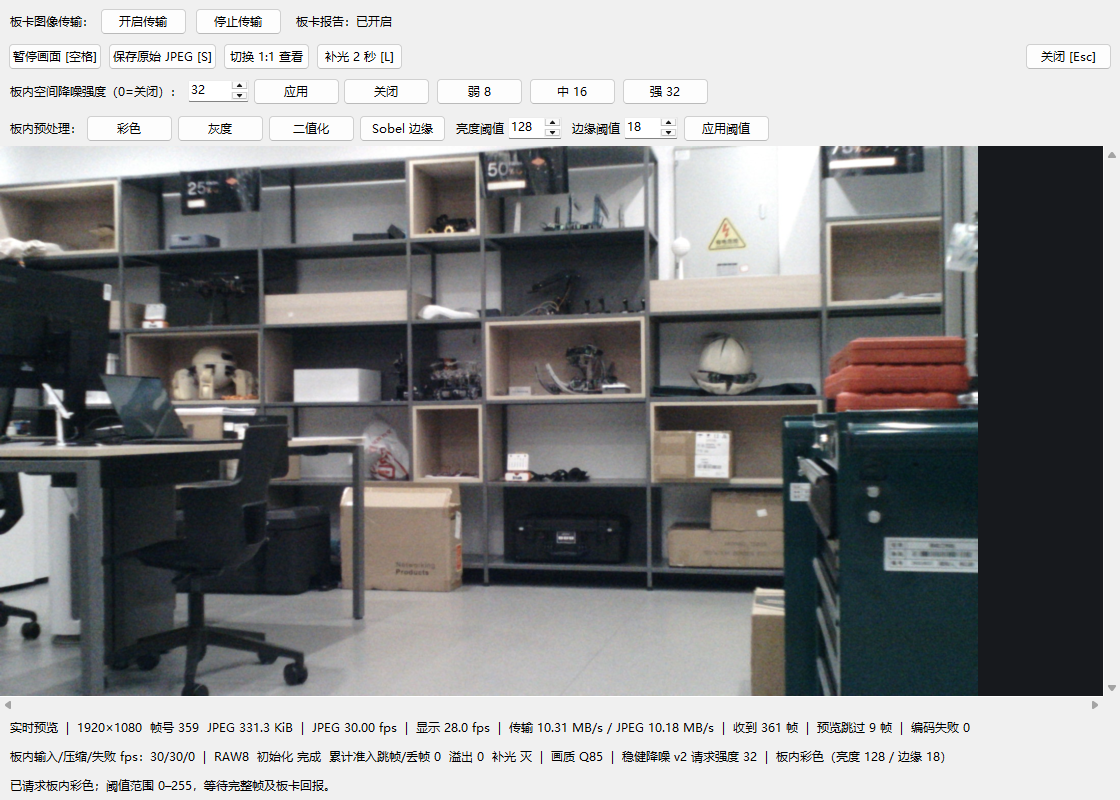
\includegraphics[width=.82\linewidth]{mode_color_window.png}
\caption{彩色模式，Q85，N32。置物架、设备和地面的颜色与亮度层次均可辨认。截图时 JPEG 331.3 KiB；稳定窗口 JPEG 载荷 10.15 MB/s、USB 接收 10.27 MB/s。}\label{fig:live-color}
\end{figure}
\begin{figure}[H]\centering
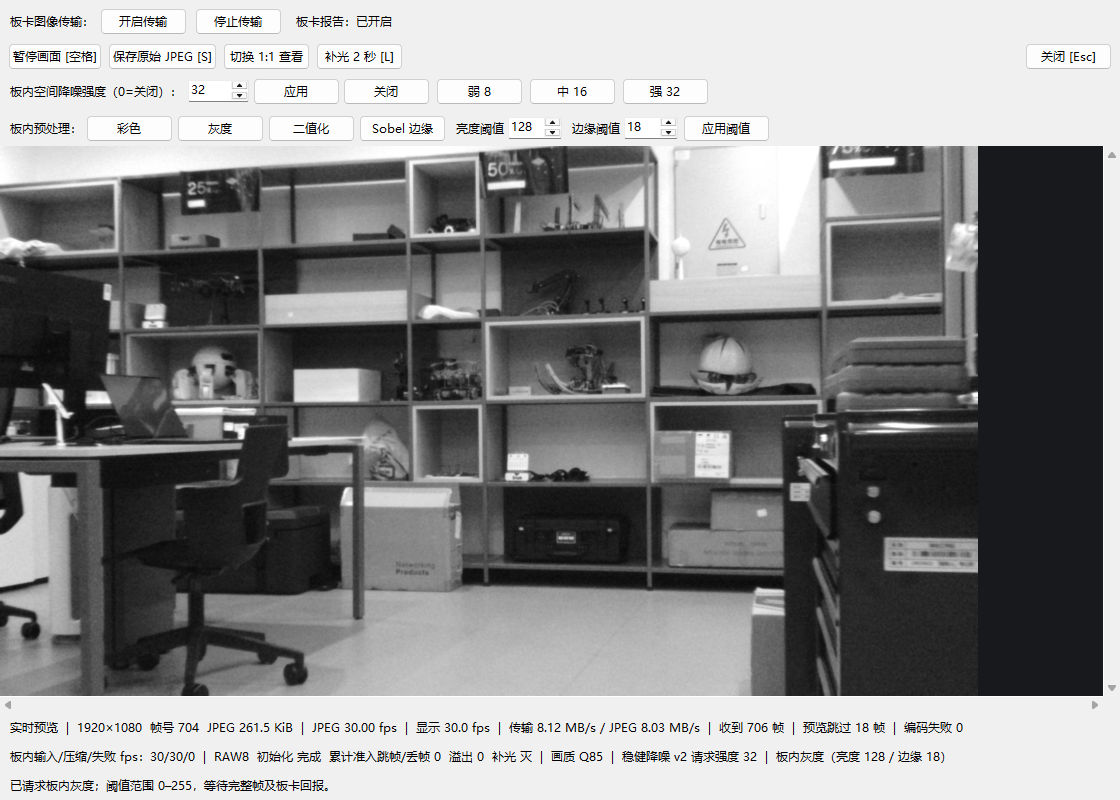
\includegraphics[width=.82\linewidth]{mode_gray_window.png}
\caption{灰度模式，Q85，N32。场景空间结构保留，色彩信息转为亮度层次。截图时 JPEG 261.5 KiB；稳定窗口 JPEG 载荷 8.05 MB/s、USB 接收 8.15 MB/s。}\label{fig:live-gray}
\end{figure}
\clearpage
\subsection{二值化阈值对比的判读}
二值化在板内比较像素亮度与阈值：$Y_{\rm out}=255$ 当 $Y\geq T_b$，否则输出 0，并将色度置为中性。提高 $T_b$ 后，只有更亮的区域保留为白色。本次选取 64～224 的六档设置，以覆盖大面积亮区、主要物体分割及高亮区域筛选。

以下各页分别显示两档真实窗口。低阈值下置物架、地面等大面积区域可能连成白块；阈值升高时较暗的隔板、设备和背景逐渐转黑，高阈值主要保留强亮区。JPEG 为有损编码，二值边界在解码后可能出现灰色过渡或轻微振铃，不能只据此判断 FPGA 比较逻辑错误。

\begin{table}[H]\centering\caption{二值化各阈值的实测载荷}\label{tab:binaryrates}
\small\begin{tabular}{@{}rrrrr@{}}\toprule
$T_b$ & 样本帧数 & 平均 JPEG (kB) & JPEG (MB/s) & USB 接收 (MB/s)\\\midrule
64 & 244 & 262.95 & 7.897 & 7.992\\
96 & 242 & 279.41 & 8.387 & 8.488\\
128 & 241 & 230.25 & 6.910 & 7.000\\
160 & 242 & 166.14 & 4.977 & 5.038\\
192 & 244 & 144.63 & 4.353 & 4.406\\
224 & 244 & 83.89 & 2.519 & 2.551\\
\bottomrule\end{tabular}\end{table}
白色面积不是码率的唯一决定因素；边界数量、形状和图像高频成分也会影响 JPEG 大小。中间阈值可能产生较复杂的明暗分界，载荷不要求随阈值单调变化。
\clearpage
\subsection{二值化阈值 64 与 96}
\begin{figure}[H]\centering
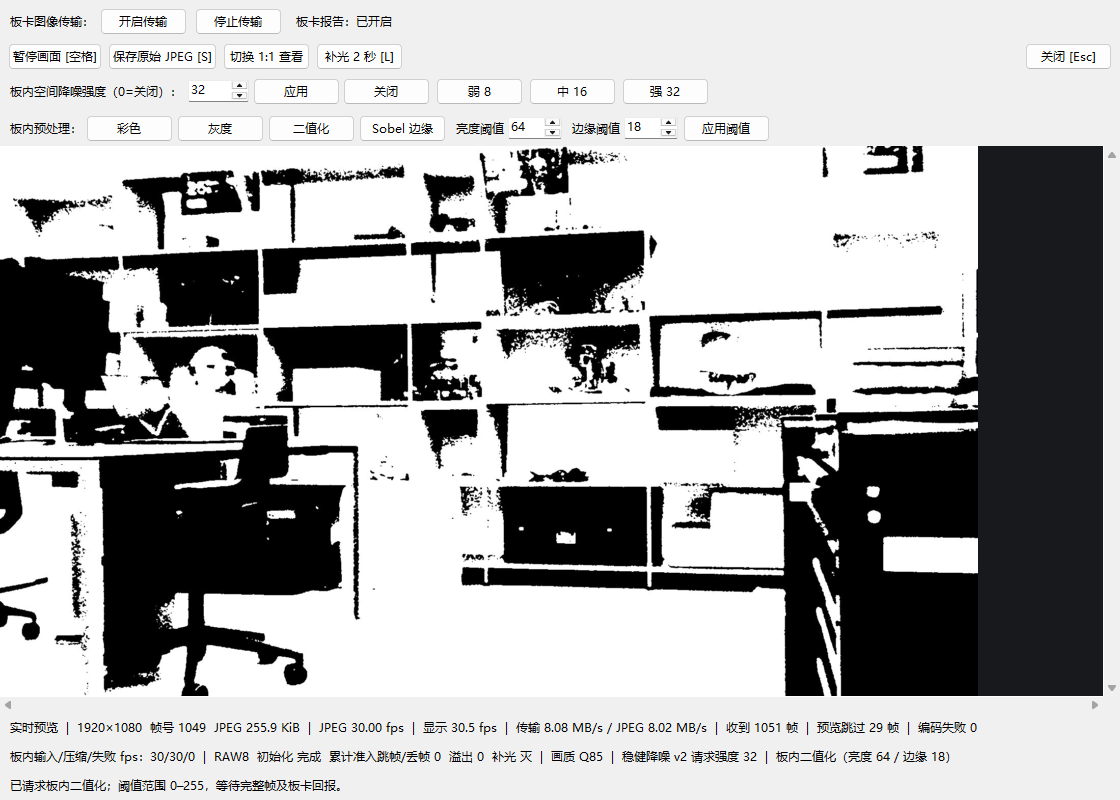
\includegraphics[width=.82\linewidth]{binary_t064_window.png}
\caption{二值化，$T_b=64$，Q85，N32。截图时 JPEG 255.9 KiB；稳定窗口 JPEG 载荷 7.90 MB/s、USB 接收 7.99 MB/s。}\label{fig:binary-64}
\end{figure}
\begin{figure}[H]\centering
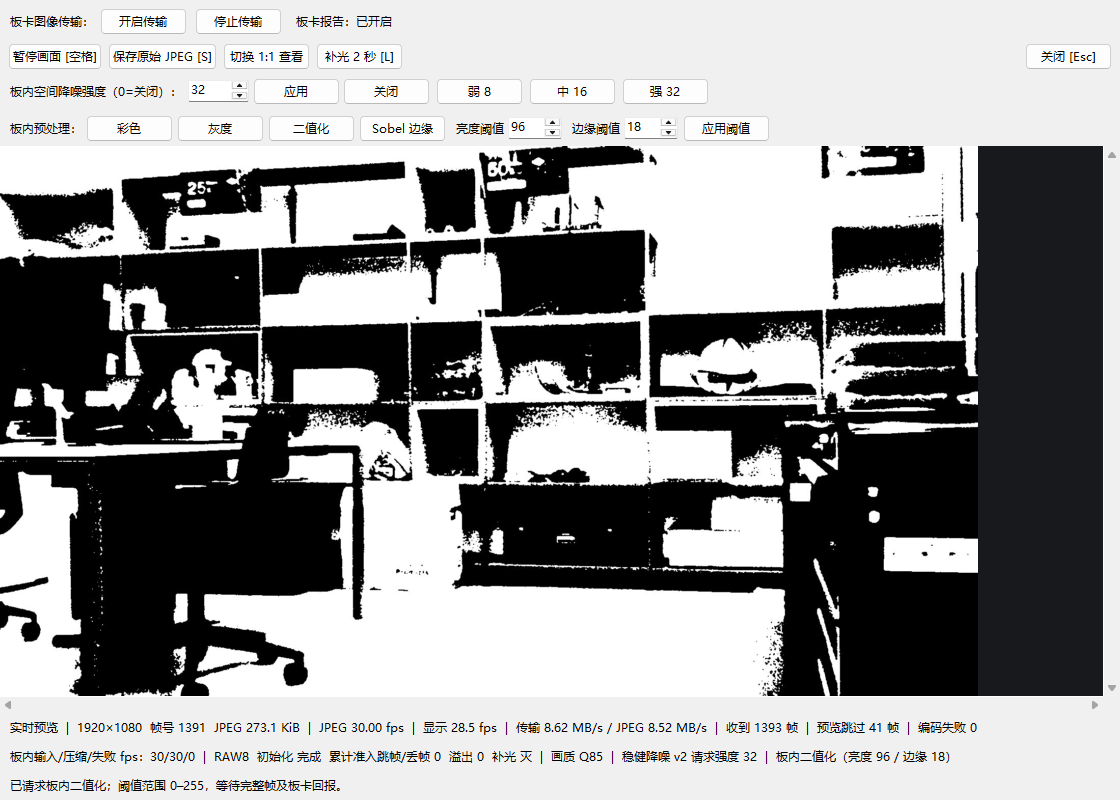
\includegraphics[width=.82\linewidth]{binary_t096_window.png}
\caption{二值化，$T_b=96$，Q85，N32。截图时 JPEG 273.1 KiB；稳定窗口 JPEG 载荷 8.39 MB/s、USB 接收 8.49 MB/s。}\label{fig:binary-96}
\end{figure}
\clearpage
\subsection{二值化阈值 128 与 160}
\begin{figure}[H]\centering
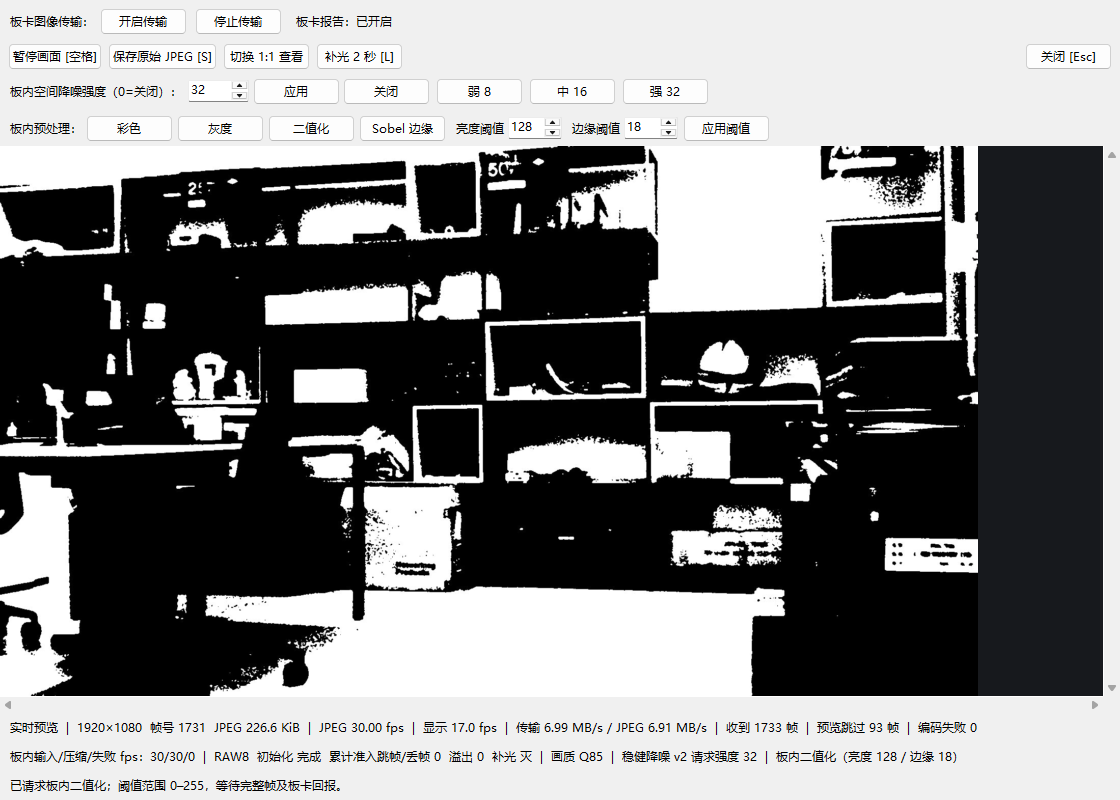
\includegraphics[width=.82\linewidth]{binary_t128_window.png}
\caption{二值化，$T_b=128$，Q85，N32。截图时 JPEG 226.6 KiB；稳定窗口 JPEG 载荷 6.91 MB/s、USB 接收 7.00 MB/s。}\label{fig:binary-128}
\end{figure}
\begin{figure}[H]\centering
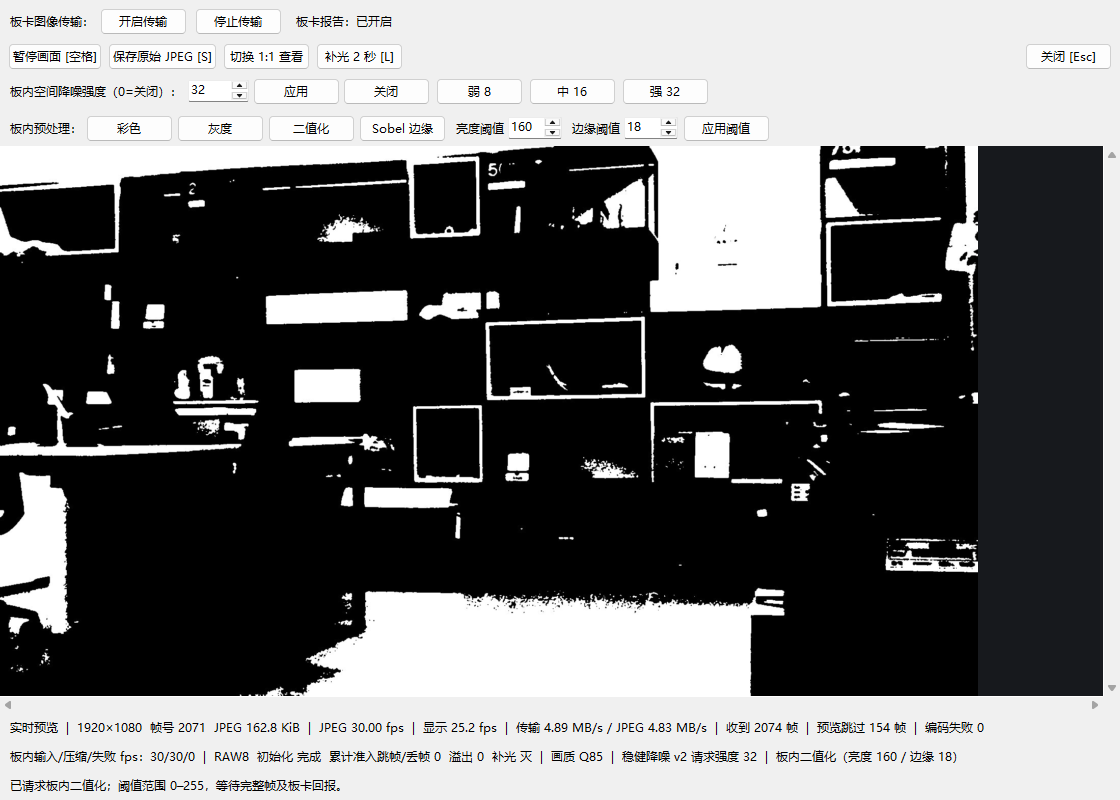
\includegraphics[width=.82\linewidth]{binary_t160_window.png}
\caption{二值化，$T_b=160$，Q85，N32。截图时 JPEG 162.8 KiB；稳定窗口 JPEG 载荷 4.98 MB/s、USB 接收 5.04 MB/s。}\label{fig:binary-160}
\end{figure}
\clearpage
\subsection{二值化阈值 192 与 224}
\begin{figure}[H]\centering
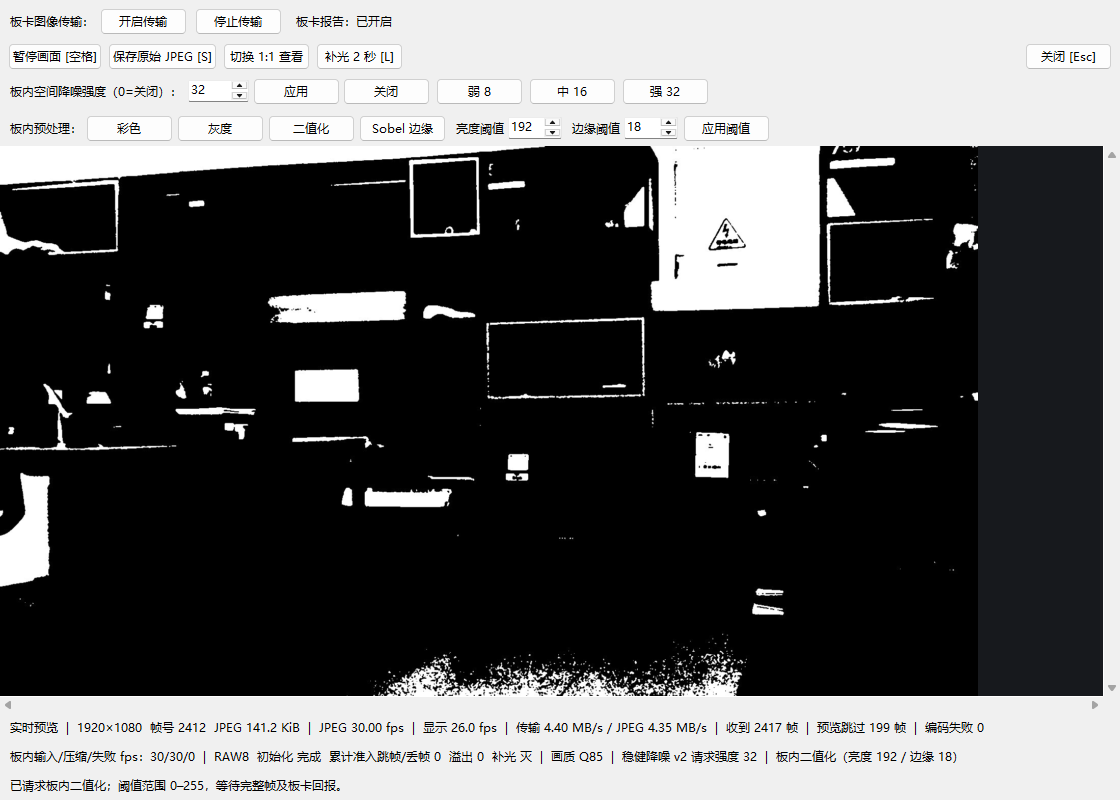
\includegraphics[width=.82\linewidth]{binary_t192_window.png}
\caption{二值化，$T_b=192$，Q85，N32。截图时 JPEG 141.2 KiB；稳定窗口 JPEG 载荷 4.35 MB/s、USB 接收 4.41 MB/s。}\label{fig:binary-192}
\end{figure}
\begin{figure}[H]\centering
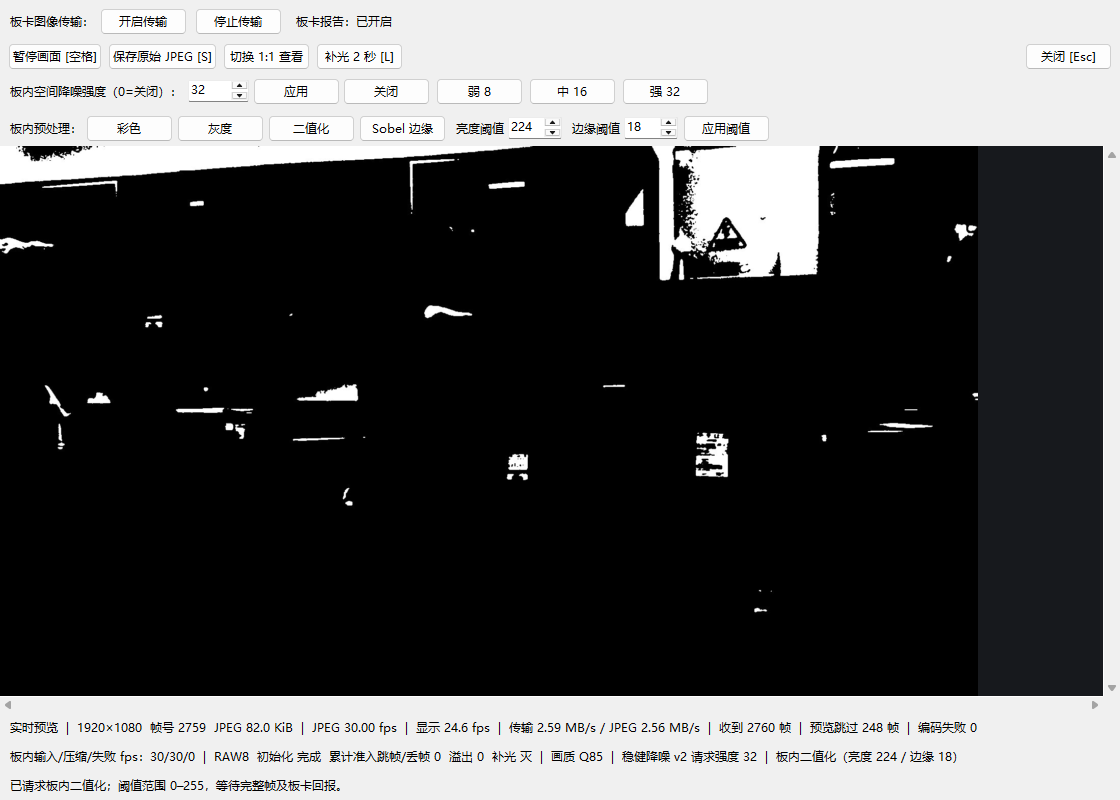
\includegraphics[width=.82\linewidth]{binary_t224_window.png}
\caption{二值化，$T_b=224$，Q85，N32。截图时 JPEG 82.0 KiB；稳定窗口 JPEG 载荷 2.52 MB/s、USB 接收 2.55 MB/s。}\label{fig:binary-224}
\end{figure}
\clearpage
\subsection{Sobel 阈值对比的判读}
当前 RTL 计算 $G_x$ 与 $G_y$ 后，使用
\[
 E=\min\!\left(255,\left\lfloor\frac{|G_x|+|G_y|+2}{4}\right\rfloor\right),
 \qquad Y_{\rm out}=\begin{cases}E,&E\geq T_e,\\0,&E<T_e.\end{cases}
\]
边缘模式保留超过阈值的梯度幅度，并不把每个边缘像素放大成纯白色。因此截图中的轮廓呈不同亮度，高阈值画面变暗也是符合实现的结果。

$T_e=8$ 能显示较多隔板、椅背、纸箱及细小纹理，但也容易保留弱变化；提高到 18、32 后，弱边缘减少；64 主要留下较强的亮度跃迁，部分连续轮廓会变细或中断。阈值应结合实际照度和目标边缘强度选择，不能只凭图像亮度高低判断检测质量。

\begin{table}[H]\centering\caption{Sobel 各阈值的实测载荷}\label{tab:edgerates}
\small\begin{tabular}{@{}rrrrr@{}}\toprule
$T_e$ & 样本帧数 & 平均 JPEG (kB) & JPEG (MB/s) & USB 接收 (MB/s)\\\midrule
8 & 240 & 293.20 & 8.778 & 8.884\\
18 & 243 & 200.69 & 6.037 & 6.101\\
32 & 244 & 173.00 & 5.184 & 5.247\\
64 & 240 & 93.24 & 2.797 & 2.832\\
\bottomrule\end{tabular}\end{table}
\src{mjpeg/rtl/camera/yuv422_preprocess.v}
\clearpage
\subsection{Sobel 边缘阈值 8 与 18}
\begin{figure}[H]\centering
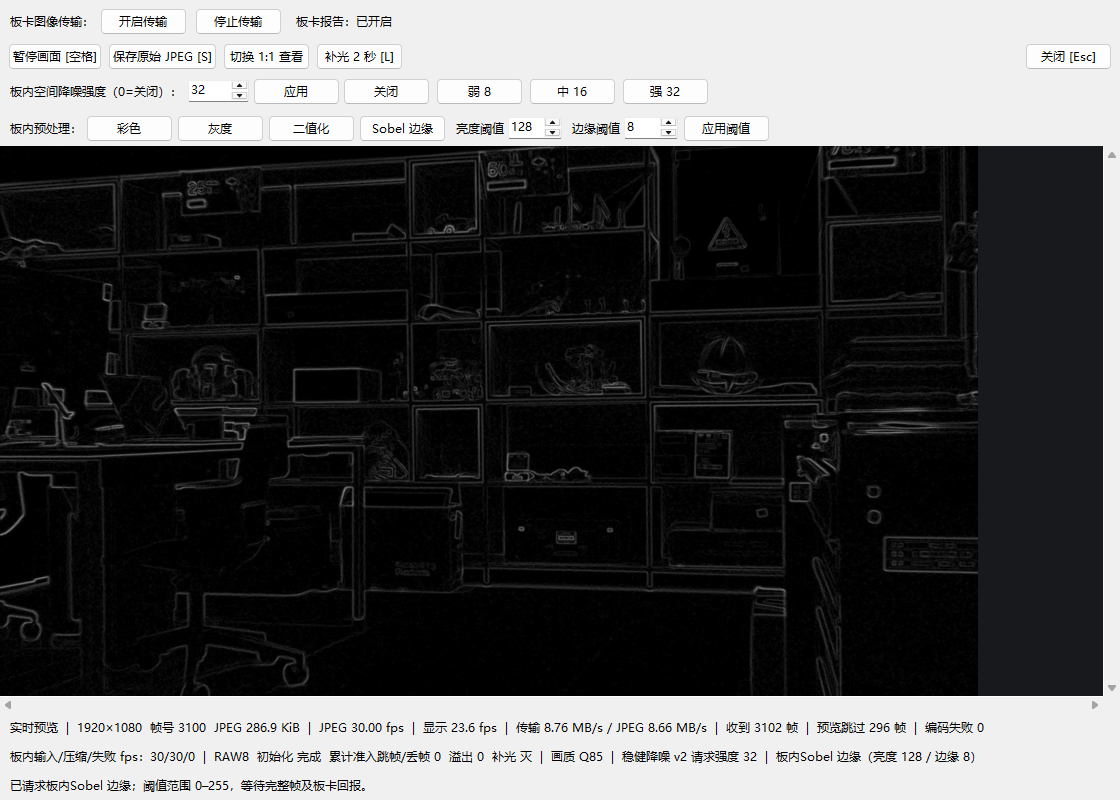
\includegraphics[width=.82\linewidth]{sobel_t008_window.png}
\caption{Sobel 边缘，$T_e=8$，Q85，N32。截图时 JPEG 286.9 KiB；稳定窗口 JPEG 载荷 8.78 MB/s、USB 接收 8.88 MB/s。}\label{fig:edge-8}
\end{figure}
\begin{figure}[H]\centering
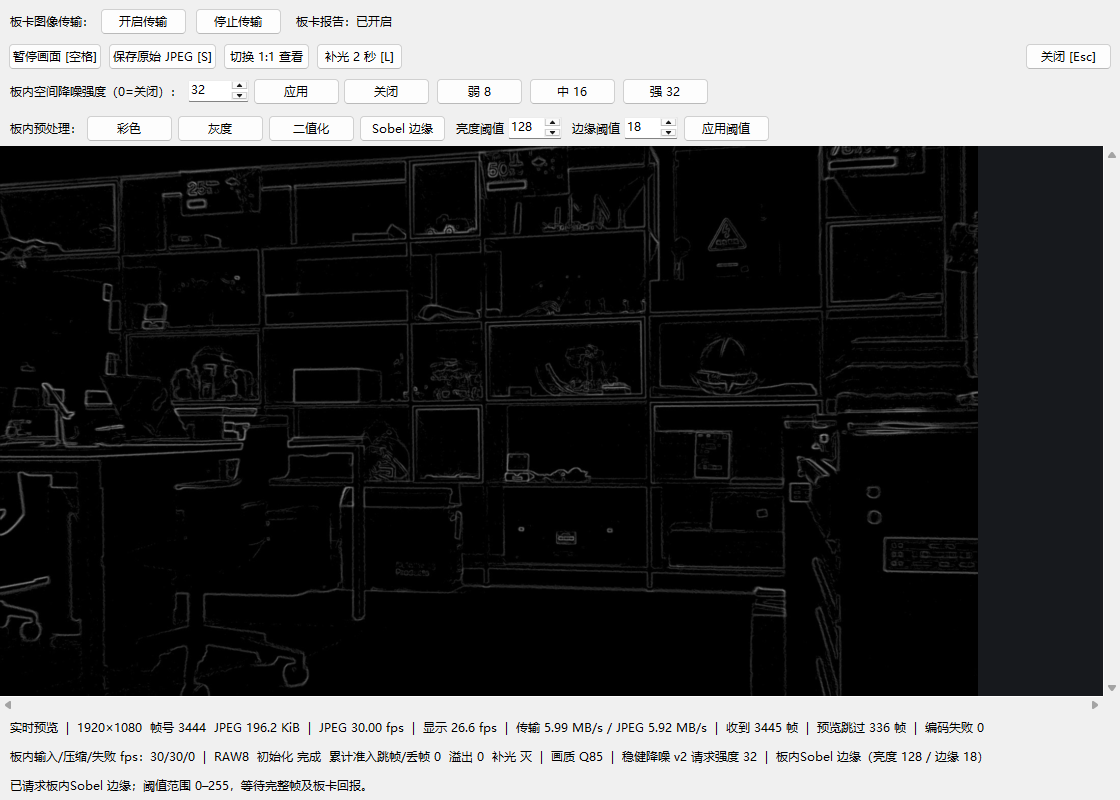
\includegraphics[width=.82\linewidth]{sobel_t018_window.png}
\caption{Sobel 边缘，$T_e=18$，Q85，N32。截图时 JPEG 196.2 KiB；稳定窗口 JPEG 载荷 6.04 MB/s、USB 接收 6.10 MB/s。}\label{fig:edge-18}
\end{figure}
\clearpage
\subsection{Sobel 边缘阈值 32 与 64}
\begin{figure}[H]\centering
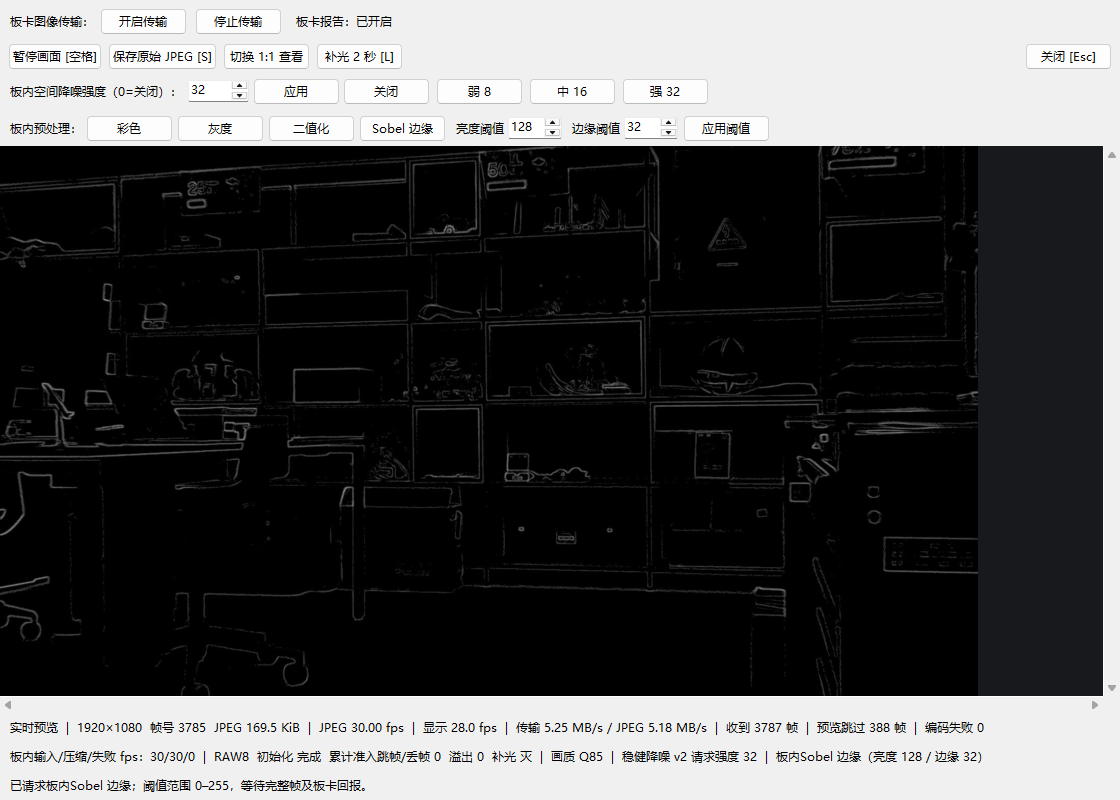
\includegraphics[width=.82\linewidth]{sobel_t032_window.png}
\caption{Sobel 边缘，$T_e=32$，Q85，N32。截图时 JPEG 169.5 KiB；稳定窗口 JPEG 载荷 5.18 MB/s、USB 接收 5.25 MB/s。}\label{fig:edge-32}
\end{figure}
\begin{figure}[H]\centering
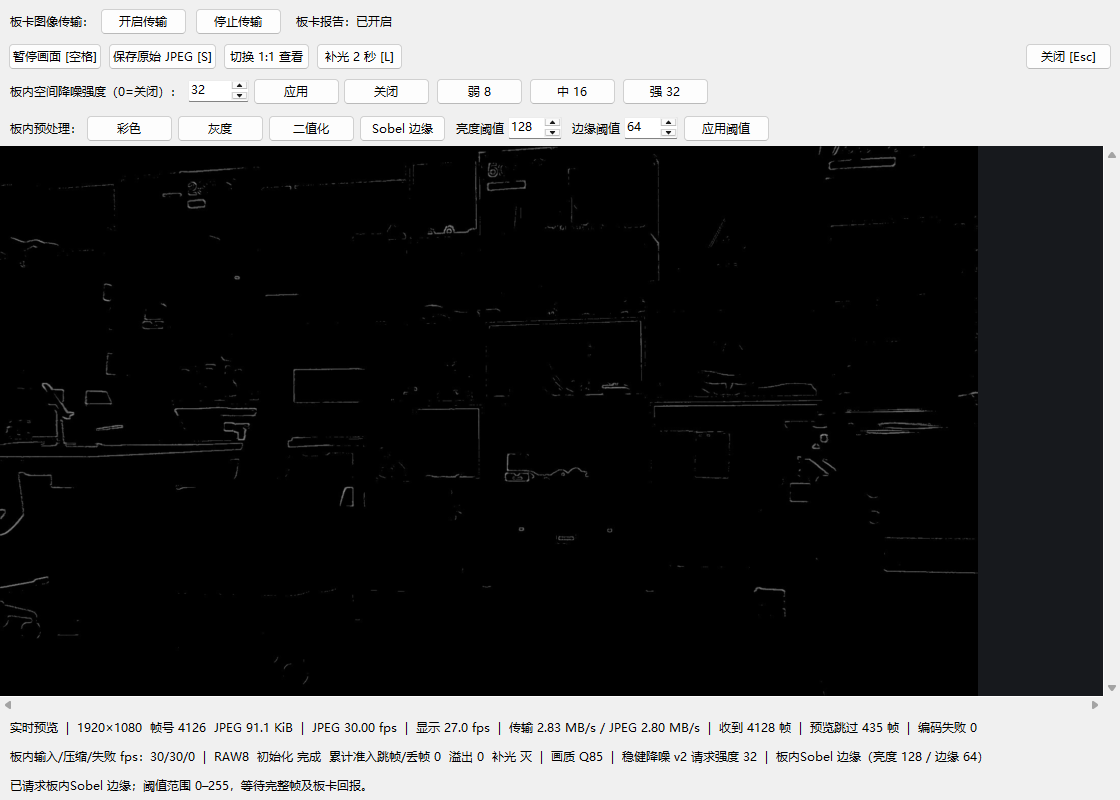
\includegraphics[width=.82\linewidth]{sobel_t064_window.png}
\caption{Sobel 边缘，$T_e=64$，Q85，N32。截图时 JPEG 91.1 KiB；稳定窗口 JPEG 载荷 2.80 MB/s、USB 接收 2.83 MB/s。}\label{fig:edge-64}
\end{figure}
\clearpage


\section{载荷、压缩效果与降噪观察}
\subsection{三档画质与本次实测带宽}
Q60、Q75、Q85 是本工程 JPEG 量化表的质量档位。较高 Q 通常保留更多量化后的细节，并增加 JPEG 大小；Q 值本身不是百分比压缩率。实际压缩比必须由原始有效载荷与压缩后的字节数计算，并注明原始格式。

本次在同一实验室场景、N32、彩色模式下依次测量三档画质，末尾再次测量 Q60，检查分时采集的场景漂移。每档切换后确认状态读回并等待稳定，采样约 12 s。下表使用十进制单位 $1\,\mathrm{kB}=1000$ B、$1\,\mathrm{MB}=10^6$ B；界面单帧大小使用 KiB，$1\,\mathrm{KiB}=1024$ B。

\begin{table}[H]\centering\caption{同场景 JPEG 质量与带宽实测}\label{tab:livequality}
\small\begin{tabular}{@{}lrrrrr@{}}\toprule
画质 & 样本帧数 & 均值 (kB/帧) & JPEG (MB/s) & USB (MB/s) & 压缩比\\\midrule
Q60 & 362 & 172.45 & 5.175 & 5.238 & 24.05:1\\
Q75 & 361 & 239.68 & 7.182 & 7.269 & 17.30:1\\
Q85 & 364 & 339.34 & 10.203 & 10.325 & 12.22:1\\
Q60 复测 & 363 & 172.27 & 5.178 & 5.241 & 24.07:1\\
\bottomrule\end{tabular}\end{table}

\begin{figure}[H]\centering
\begin{tikzpicture}
\begin{axis}[width=.88\linewidth,height=5.8cm,ybar,bar width=14pt,
 ymin=0,ylabel={带宽 (MB/s)},symbolic x coords={Q60,Q75,Q85},xtick=data,
 ymajorgrids=true,grid style={gray!20},legend style={at={(0.5,1.03)},anchor=south,legend columns=2,draw=none,column sep=8pt},
 legend image code/.code={\draw[#1] (0cm,-.1cm) rectangle (.28cm,.1cm);},
 enlarge x limits=.23]
\addplot[fill=teal!65,draw=teal] coordinates {(Q60,5.175) (Q75,7.182) (Q85,10.203)};
\addplot[fill=gray!45,draw=gray] coordinates {(Q60,5.238) (Q75,7.269) (Q85,10.325)};
\legend{JPEG 有效载荷,USB 接收记录}
\end{axis}\end{tikzpicture}
\caption{本次实测质量档位与带宽关系。帧率均约 30 fps，USB 读出记录包含 MBLK 开销。}\label{fig:livebandwidth}
\end{figure}
本次场景中，从 Q85 调低至 Q60，JPEG 平均载荷率从 10.203 MB/s 降至 5.175 MB/s，减少约 49.3\%。末尾 Q60 复测为 5.178 MB/s，相对首次变化 +0.04\%，用于提示分时统计的波动范围；不作为同输入压缩的严格误差界限。
\clearpage
\subsection{Q60 与 Q75 的界面带宽对照}
\begin{figure}[H]\centering
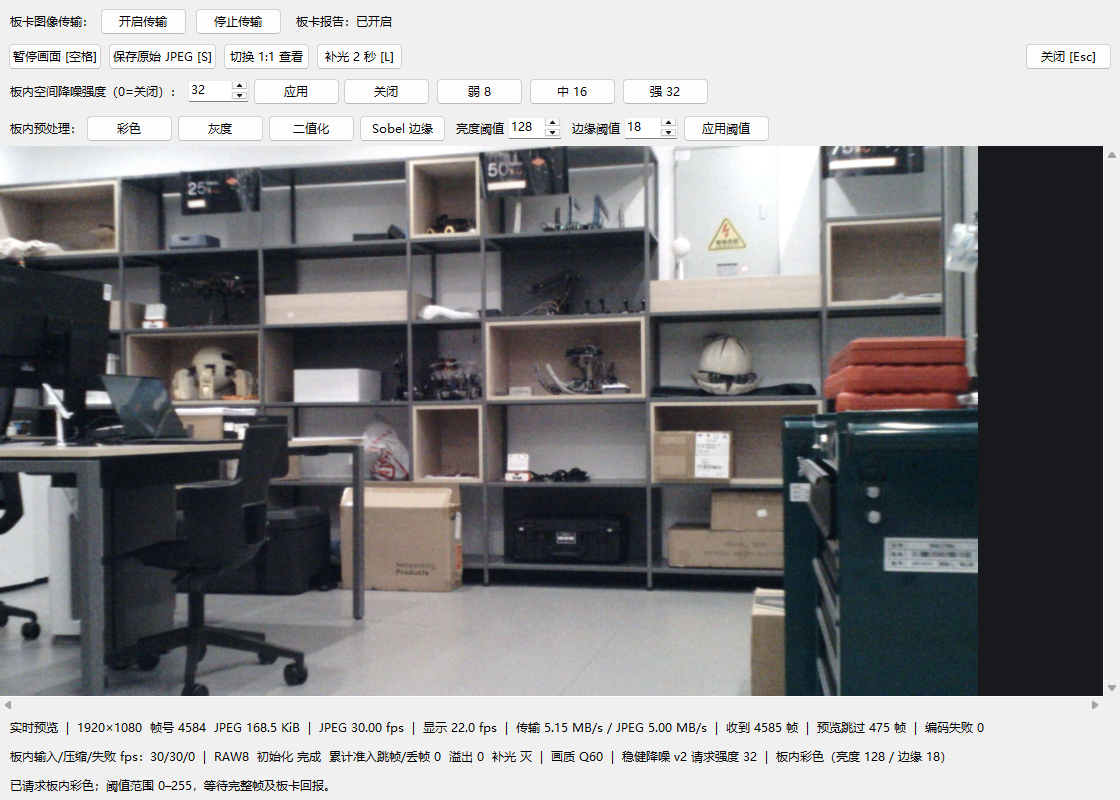
\includegraphics[width=.82\linewidth]{quality_q60_window.png}
\caption{彩色 Q60，N32。较低质量档位减少本场景的编码字节数。截图时 JPEG 168.5 KiB；稳定窗口 JPEG 载荷 5.18 MB/s、USB 接收 5.24 MB/s。}\label{fig:quality60}
\end{figure}
\begin{figure}[H]\centering
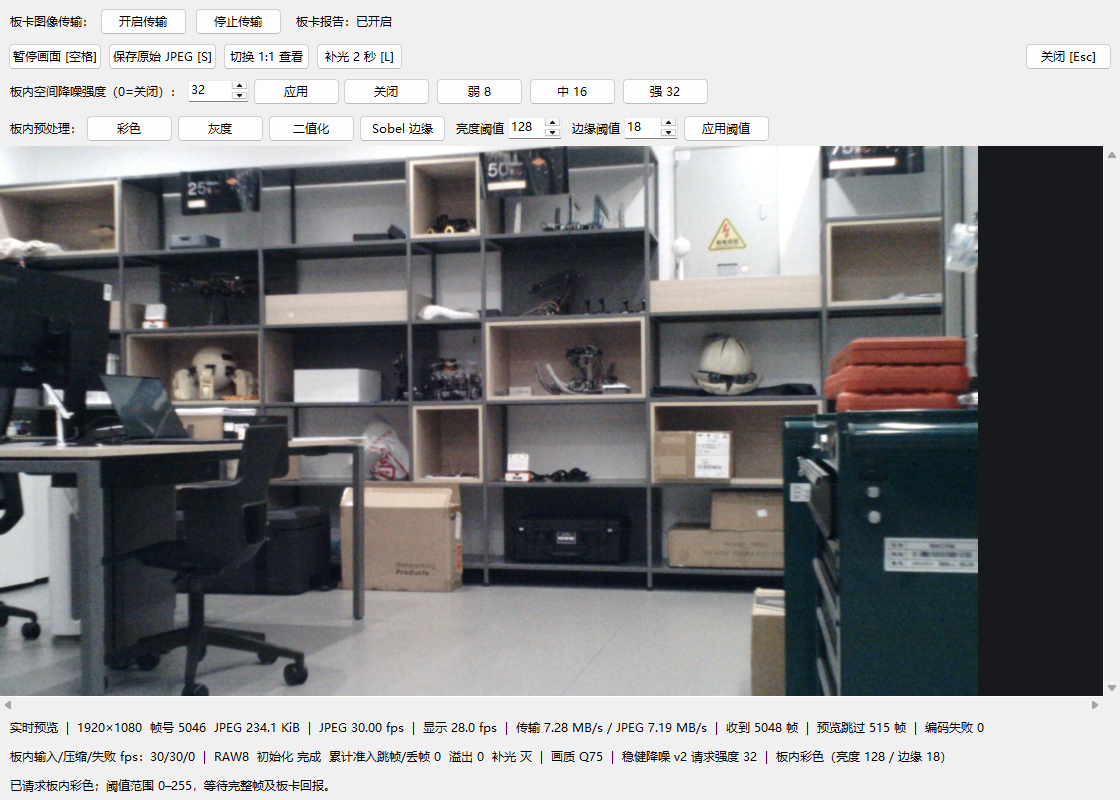
\includegraphics[width=.82\linewidth]{quality_q75_window.png}
\caption{彩色 Q75，N32。底部状态同时显示质量、帧大小、帧率和传输带宽。截图时 JPEG 234.1 KiB；稳定窗口 JPEG 载荷 7.18 MB/s、USB 接收 7.27 MB/s。}\label{fig:quality75}
\end{figure}
\clearpage
\subsection{Q85 与 Q60 复测的界面对照}
\begin{figure}[H]\centering
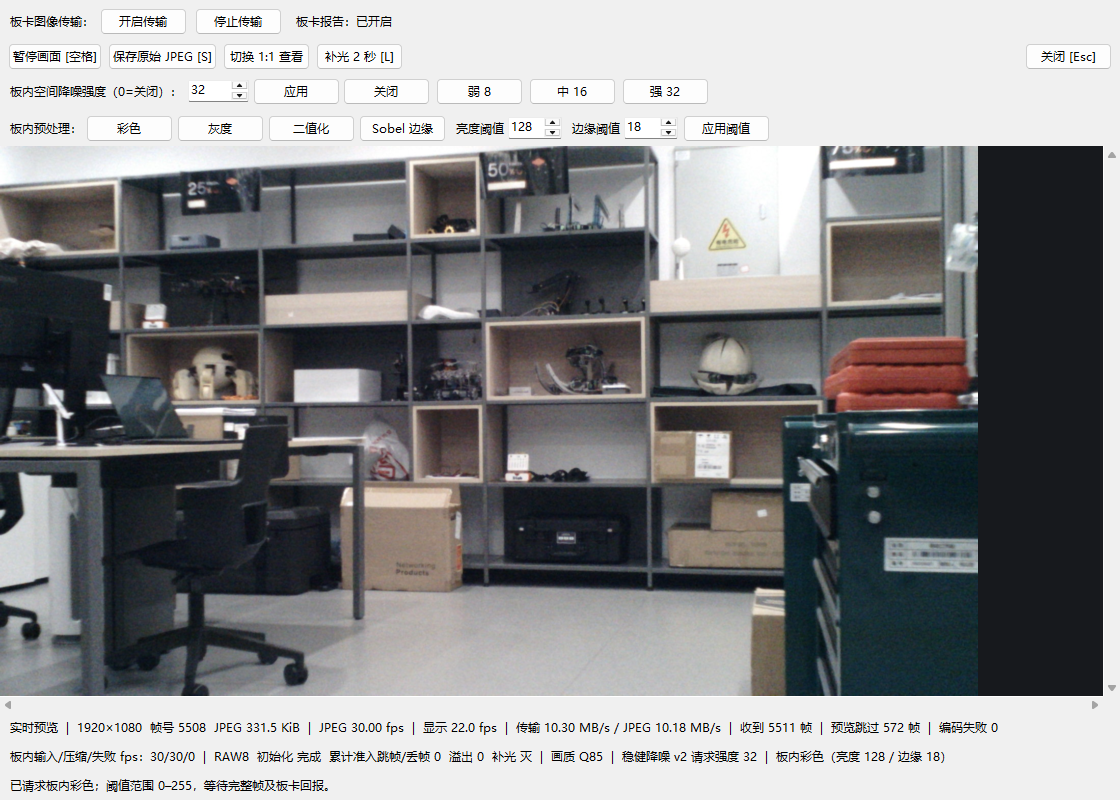
\includegraphics[width=.82\linewidth]{quality_q85_window.png}
\caption{彩色 Q85，N32。本次场景中载荷高于 Q60 和 Q75。截图时 JPEG 331.5 KiB；稳定窗口 JPEG 载荷 10.20 MB/s、USB 接收 10.32 MB/s。}\label{fig:quality85}
\end{figure}
\begin{figure}[H]\centering
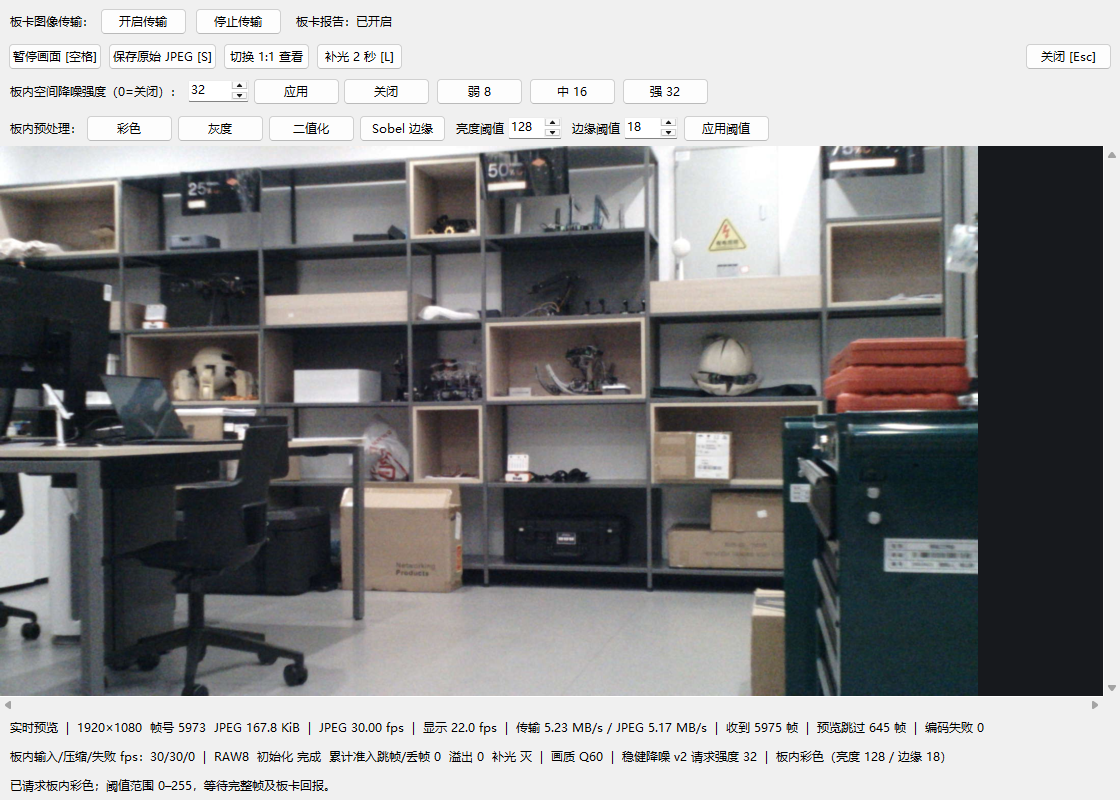
\includegraphics[width=.82\linewidth]{quality_q60_repeat_window.png}
\caption{返回彩色 Q60 复测，N32。检查本次分时采集的载荷漂移。截图时 JPEG 167.8 KiB；稳定窗口 JPEG 载荷 5.18 MB/s、USB 接收 5.24 MB/s。}\label{fig:quality60-repeat}
\end{figure}
\clearpage
\subsection{压缩比与带宽口径}
以编码前 YUV422 有效像素为参照，一帧大小为
\[
 S_{\rm YUV422}=1920\times1080\times2=4\,147\,200\ \mathrm{B},\qquad
 B_{\rm raw,30}=124.416\ \mathrm{MB/s}.
\]
设稳定窗口平均 JPEG 大小为 $\overline S_{\rm JPEG}$，则
\[
 R=\frac{4\,147\,200}{\overline S_{\rm JPEG}},\qquad
 \eta=\left(1-\frac{\overline S_{\rm JPEG}}{4\,147\,200}\right)\times100\%,\qquad
 B_{\rm JPEG}\approx\overline S_{\rm JPEG}\,f/10^6.
\]
Q60 的平均 JPEG 为 172445.76 B，按 YUV422 计算压缩比 24.05:1，有效载荷减少 95.84\%。Q75 的平均 JPEG 为 239675.46 B，按 YUV422 计算压缩比 17.30:1，有效载荷减少 94.22\%。Q85 的平均 JPEG 为 339341.77 B，按 YUV422 计算压缩比 12.22:1，有效载荷减少 91.82\%。

若改用传感器 RAW8 作为参照，一帧为 $2\,073\,600$ B，相应压缩比减半；两种基准不可混写。表\ref{tab:livequality}统一采用 YUV422。当前灰度、二值化和边缘仍沿用 JPEG 颜色帧及中性色度的链路格式，视觉上单色并不意味着传输变成无损 1 bit 像素流。

统计中的 JPEG 带宽为接收的完整 JPEG 字节增量除以主机单调时钟间隔；USB 带宽为相同窗口内解析器收到的 MBLK 记录字节增量，包含分块头、帧描述和状态记录。它不包含 USB 物理层握手、总线填充等全部开销，所以不能直接等同于 USB 总线利用率，也不能用标称 USB 2.0 速率直接反推链路余量。

本次 16 个稳定窗口的编码失败、FIFO 溢出及板内准入跳帧/丢帧增量均为 0，板卡时间戳计算的帧率约为 30.0019 fps。GUI 只解码显示选中的最新帧，本次采集未声明每个接收帧都经过独立完整像素解码；逐帧完整解码验收由前述严格接收器历史测试提供。截图不能单独替代长时间稳定性测试。
\evid{evidence/quality_q60.json；quality_q75.json；quality_q85.json；quality_q60_repeat.json}
\clearpage

\subsection{历史验收的载荷与降噪对照}
\begin{figure}[H]\centering
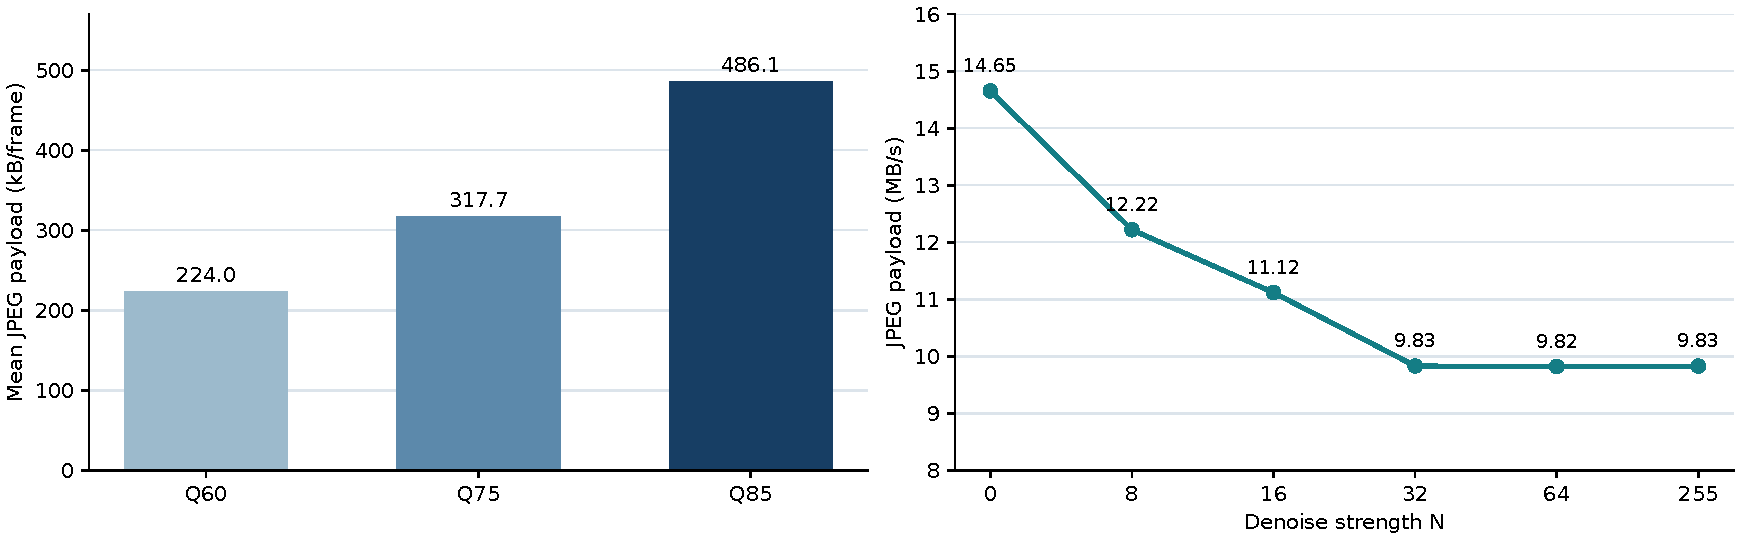
\includegraphics[width=.98\linewidth]{payload_results.pdf}
\caption{实板 JPEG 载荷。左图来自画质轮换，右图来自降噪重测前六段；均为分时实景统计。}\label{fig:payload}
\end{figure}
以下数据来自 2026 年 10 月 11 日的历史验收，场景和设置与本次演示不同。该次三档画质平均 JPEG 大小约为 224.0、317.7、486.1 kB/帧，帧率均约 30.002 fps。降噪重测中 N0 与 N32 载荷率分别约 14.654 MB/s、9.832 MB/s，下降约 32.9\%。抑制高频分量可以减小编码载荷，这种变化不能单独证明画质改善。

\begin{figure}[H]\centering
\begin{subfigure}{.485\linewidth}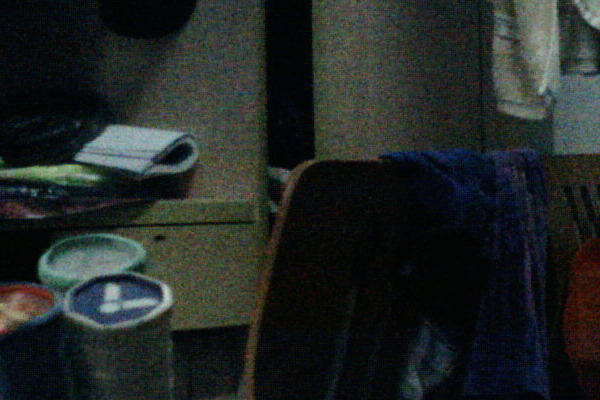
\includegraphics[width=\linewidth]{denoise_off_roi.png}\caption{N0：原样保留}\end{subfigure}\hfill
\begin{subfigure}{.485\linewidth}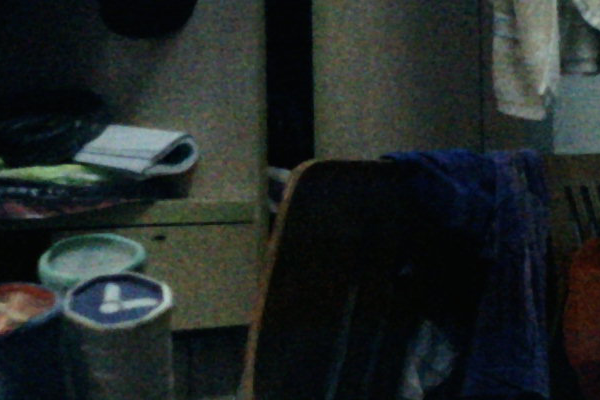
\includegraphics[width=\linewidth]{denoise_32_roi.png}\caption{N32：完整中值混合}\end{subfigure}
\caption{实拍局部对照，原图相同位置 $(500,400)$～$(1100,800)$ 裁剪，未锐化。分时采集，不作为相同输入下的定量画质比较。}\label{fig:nr}
\end{figure}
局部图中 N32 的墙面与织物色斑更平滑，部分纹理细节也可能减弱。当前缺少无噪声参考、曝光锁定和运动场景，不报告 PSNR、SSIM 或动态画质收益。

严格彩色长测使用 N32，平均 JPEG 为 326776.37 字节、约 9.804 MB/s。以 YUV422 有效载荷为基准，压缩比 12.69:1、载荷减少 92.12\%；以 RAW8 为基准则为 6.35:1、减少 84.24\%。不同原始格式必须标明计算基准，MBLK 和 USB 开销另计。
\clearpage
